\chapter{Implementacja}
\label{cha:rozdz4}

W tym rozdziale opisuję wymagania wobec projektu, który zawiera implementację gry ,,Love Letter'' i opisanych algorytmów. Następnie przedstawiam koncepcję wykonania wraz z diagramami UML, a na końcu prezentuję system i opisuję problemy napotkane w trakcie realizacji.

\section{Analiza wymagań}
Ponieważ celem pracy jest porównanie działania algorytmów gry karcianej, pierwszym krokiem potrzebnym do jego realizacji jest zaimplementowanie samej gry. Jak zostało to napisane w [\ref{bib:analiza_wymagan}], przed właściwą implementacją programu należy określić jego wymagania funkcjonalne i niefunkcjonalne. Większość wymagań jest już udokumentowana w postaci zasad gry opisanych w rozdziale \ref{cha:rozdz2}, należy jednak wyszczególnić pewne dodatkowe wymogi:
\begin{itemize}
	\item program musi udostępniać interfejs do którego można podłączyć różne algorytmy podejmujące decyzje,
	\item interfejs musi udostępniać aktualny stan gry oraz zbiór decyzji możliwych do podjęcia,
	\item interfejs musi zawierać funkcjonalność pozwalającą na utworzenie nowej instancji gry z zadanym stanem początkowym i podjętą decyzją. W nowej instancji wszystkie nieznane elementy gry są losowane na nowo (np. talia karta jest przetasowywana),
	\item program musi umożliwiać wybranie dwóch dowolnych algorytmów, które będą ze sobą grać, oraz ustawienie liczby gier które rozegrają,
	\item algorytm MCTS powinien mieć możliwość ustawienia dwóch parametrów: czasu wykonania, oraz algorytmu przeciwnika wykorzystywanego w symulacjach,
	\item po skończonej serii gier program powinien wyświetlać szczegółowe statystyki rozgrywek w formie wykresu i zapisywać dane do pliku.
\end{itemize}
Wymagania niefunkcjonalne:
\begin{itemize}
	\item program powinien uruchamiać się bez względu na środowisko.
	\item program nie powinien wymagać od użytkownika znajomości szczegółów implementacji.
	\item program powinien udostępniać instrukcje pomocy.
\end{itemize}
Do zwracanych statystyk powinny należeć:
\begin{itemize}
	\item procentowa liczba zwycięstw każdego algorytmu z wyszczególnieniem na tury w których została zakończona runda.
	\item rozkład procentowy zakończeń gry - ile rund skończyło się zagraniem karty Barona, Strażniczki, Księcia lub w ostatniej turze po wyczerpaniu talii.
	\item wyszczególnienie procentowej liczby zwycięstw w zależności od tego który algorytm wykonuje ruch jako pierwszy.
\end{itemize}


\section{Koncepcja wykonania i wykorzystane technologie}
By skupić się wyłączne na merytorycznym działaniu projektu, postanowiłem zaimplementować program w postaci aplikacji konsolowej, gdzie komunikacja odbywa się za pomocą wiersza poleceń$^{[\ref{bib:wiki_wierszPolecen}]}$. Wprowadzenie warstwy graficznej jest zbędne wobec postawionych wymagań.

Pomimo prostoty i niezmienności wymagań funkcjonalnych, projekt zostanie wykonany zgodnie z metodyką zwinną (ang. agile methodology)$^{[\ref{bib:wiki_waterfall}]}$, która wciąż zyskuje na popularności względem metodyk kaskadowych. Jej główną cechą jest porzucenie szczegółowego planowania projektu na rzecz obserwacji i reagowania. Całość oprogramowania jest wytwarzana w kolejnych iteracjach, w których implementowane są kolejne funkcjonalności, oraz testowane i poprawiane stare. Poniżej zaplanowane przeze mnie iteracje tworzenia projektu:

\begin{figure}[H]
	\centering
	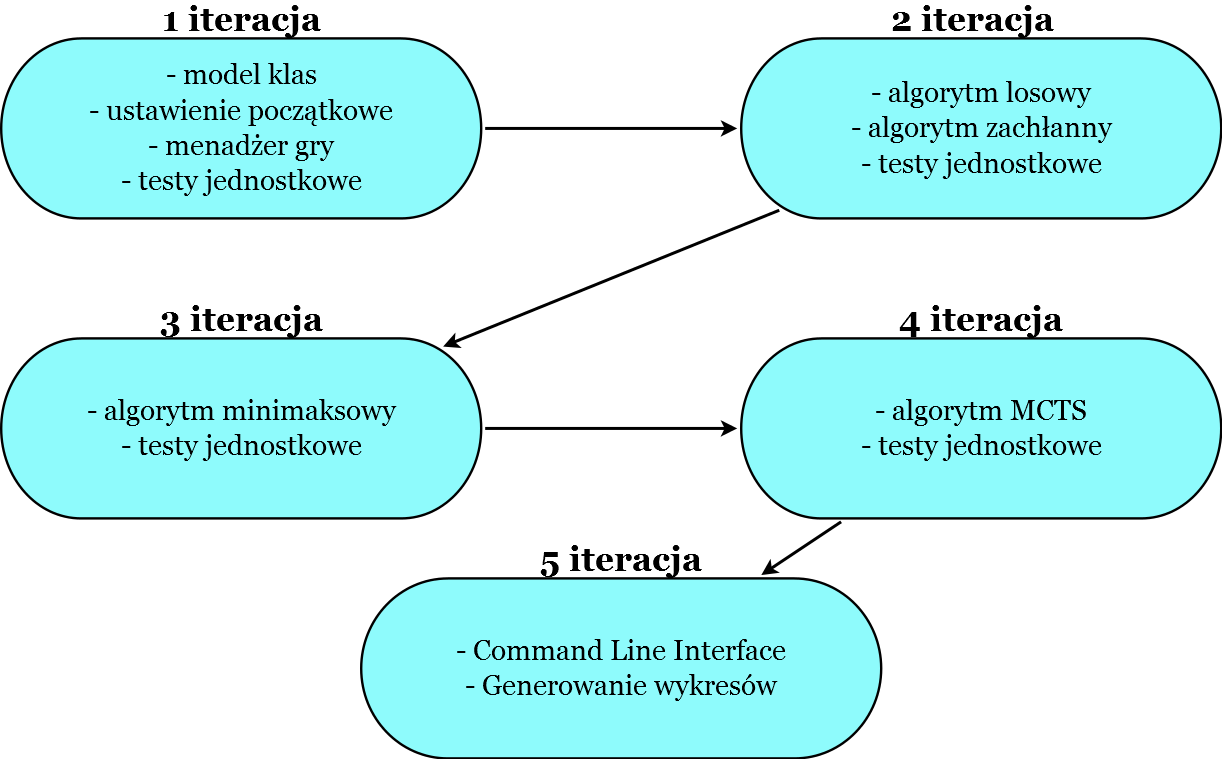
\includegraphics[width=\textwidth]{Resources/DiagramIteracji.png}
	\caption{Zaplanowane iteracje} 
	\label{fig:llMainImage}
\end{figure}

Ze względu na osobiste umiejętności, do implementacji wybrałem język programowania Java SE w wersji 8$^{[\ref{bib:java}]}$. Jest to język obiektowy, o ścisłym typowaniu, działający na maszynie wirtualnej Javy, co zapewnia kompatybilność ze wszystkimi systemami operacyjnymi. Całość projektu wykonałem w środowisku programistycznym IntelliJ IDEA w darmowej wersji Community$^{[\ref{bib:intellij}]}$.

\section{Diagramy}

\subsection{Diagram klas pakietu model}

\begin{figure}[H]
	\centering
	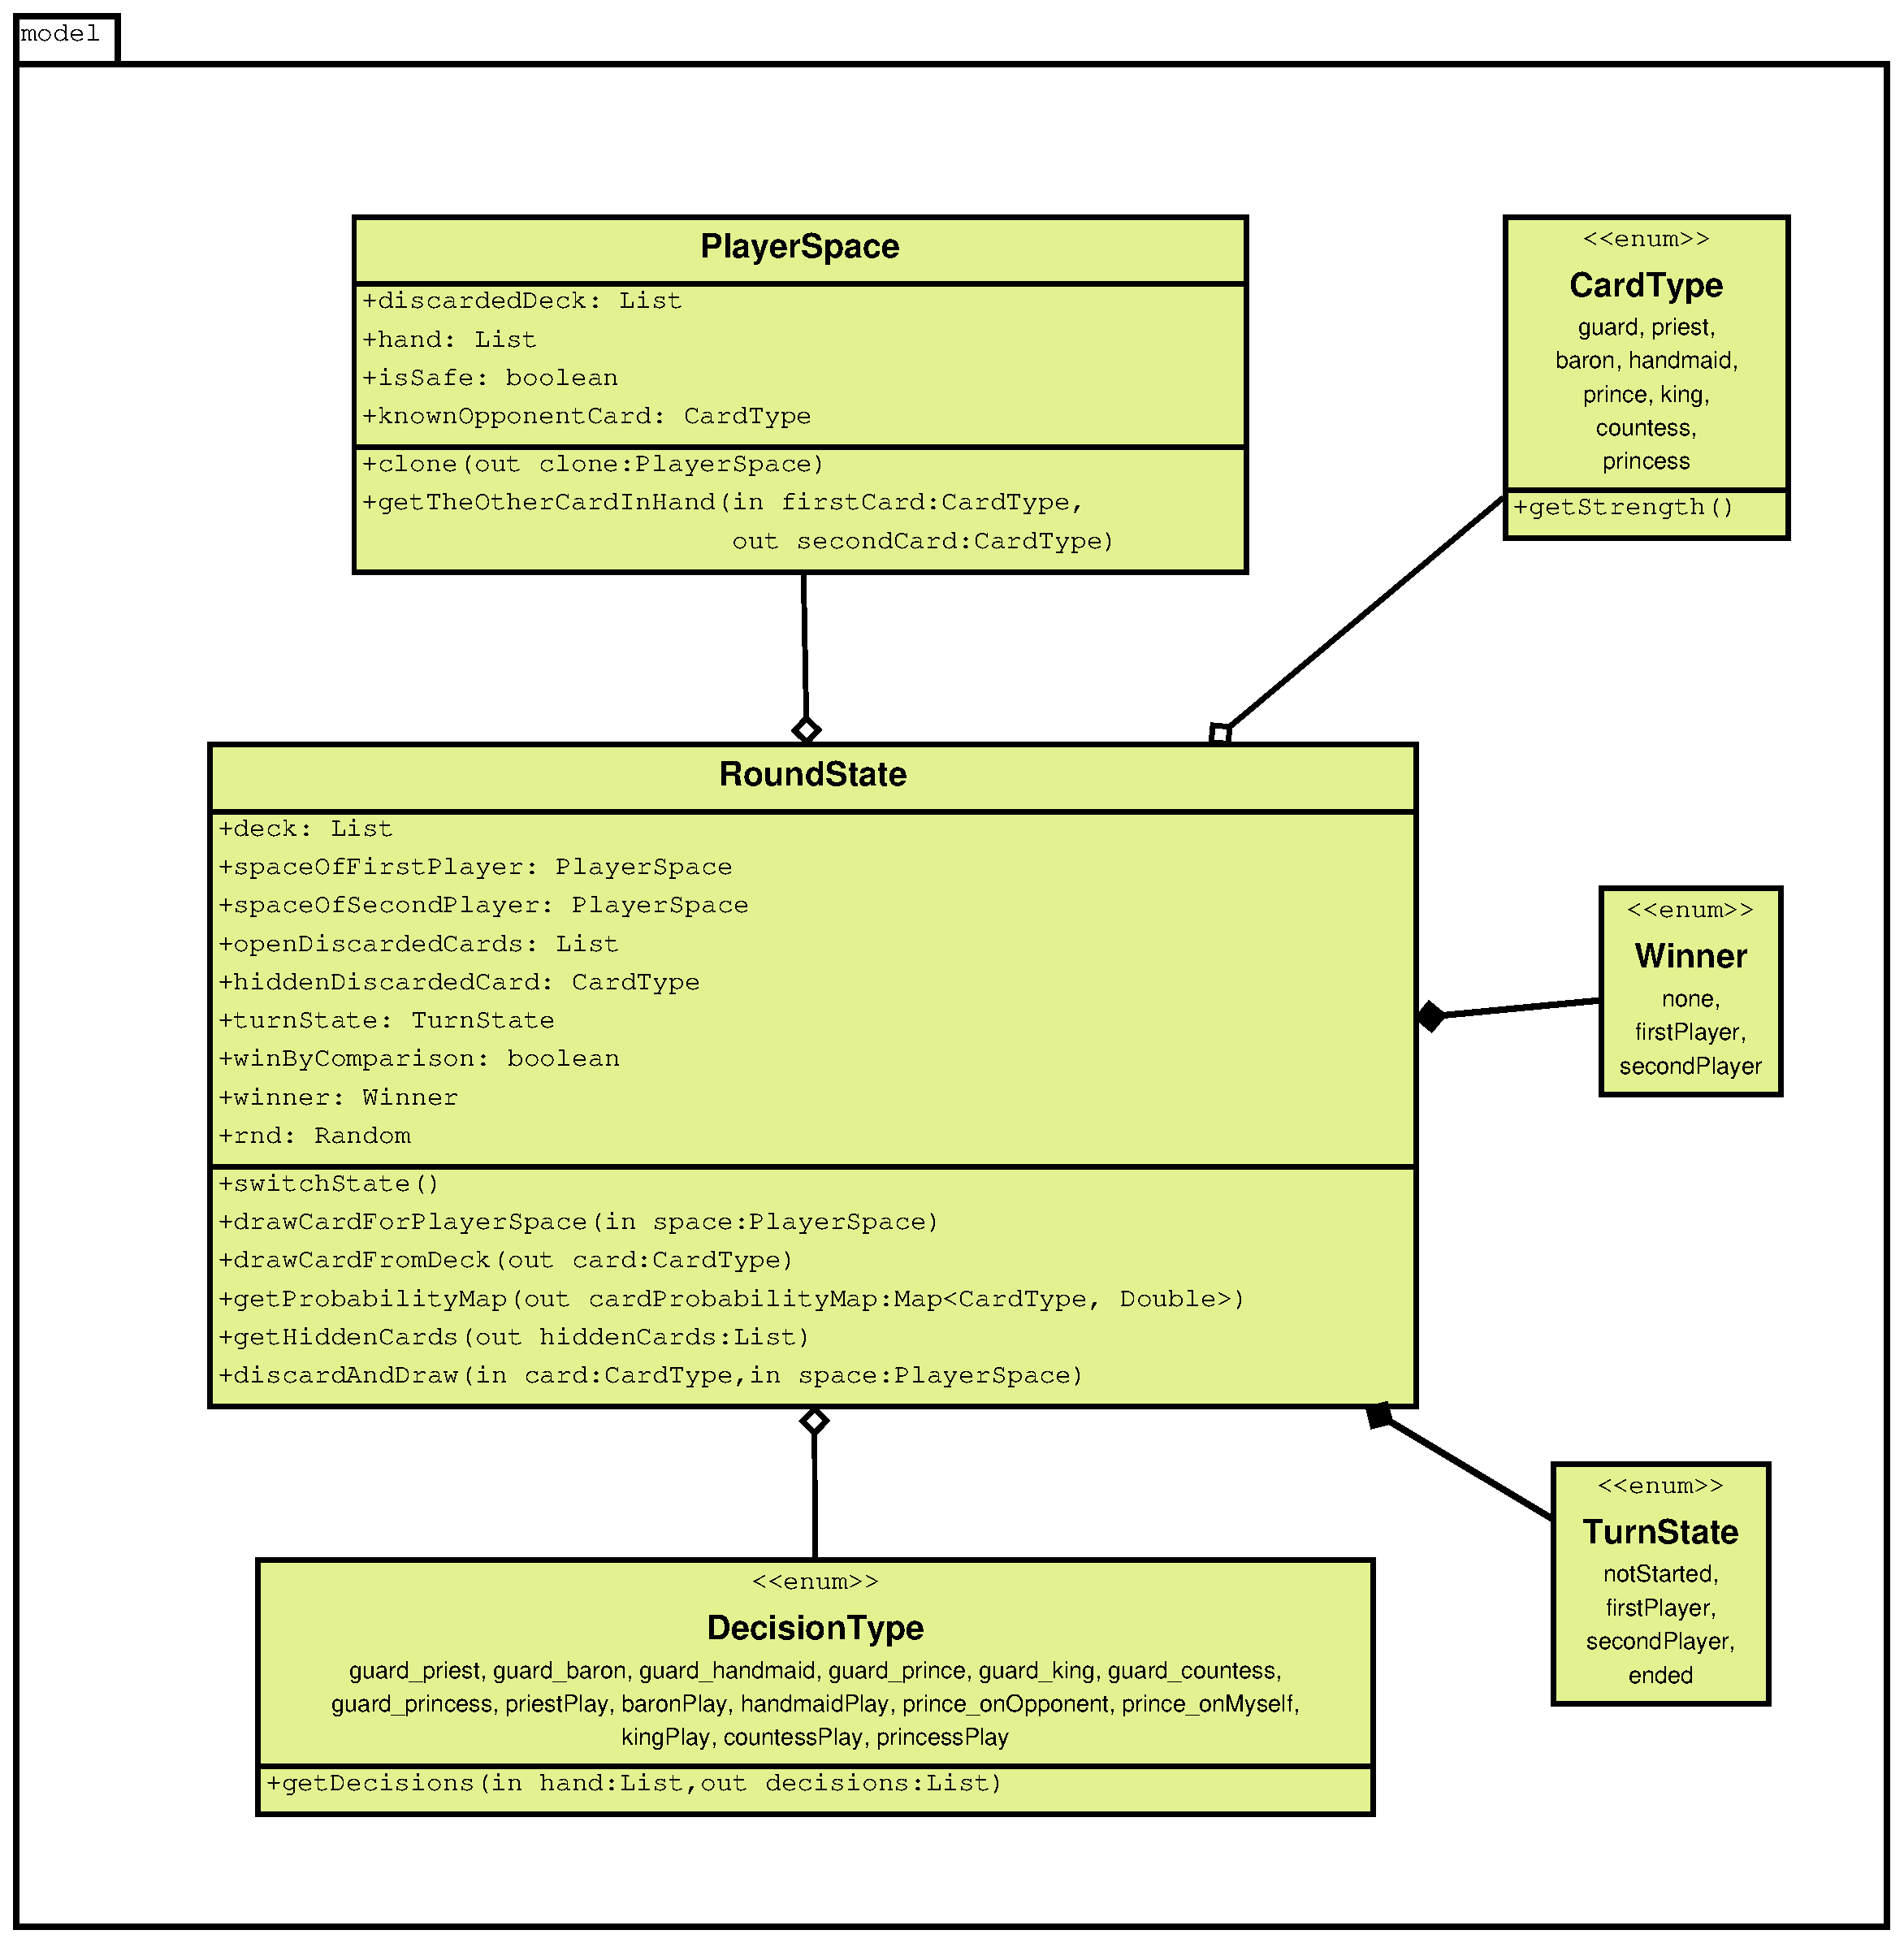
\includegraphics[width=\textwidth]{Resources/diagramKlas_model.eps}
	\caption{Diagram klas pakietu \textit{model}} 
	\label{fig:llMainImage}
\end{figure}

W danym pakiecie znajdują się wszystkie elementy składające się na samą grę. Głównym element jest klasa RoundState, odpowiadająca wierzchołkom $s_i$ należącym do zbioru $S$ modelu matematycznego. Karty oraz wynikające z nich decyzje utworzone reprezentoawne są wpostaci klas typu enum.

\subsection{Diagram klas pakietu player}

\begin{figure}[H]
	\centering
	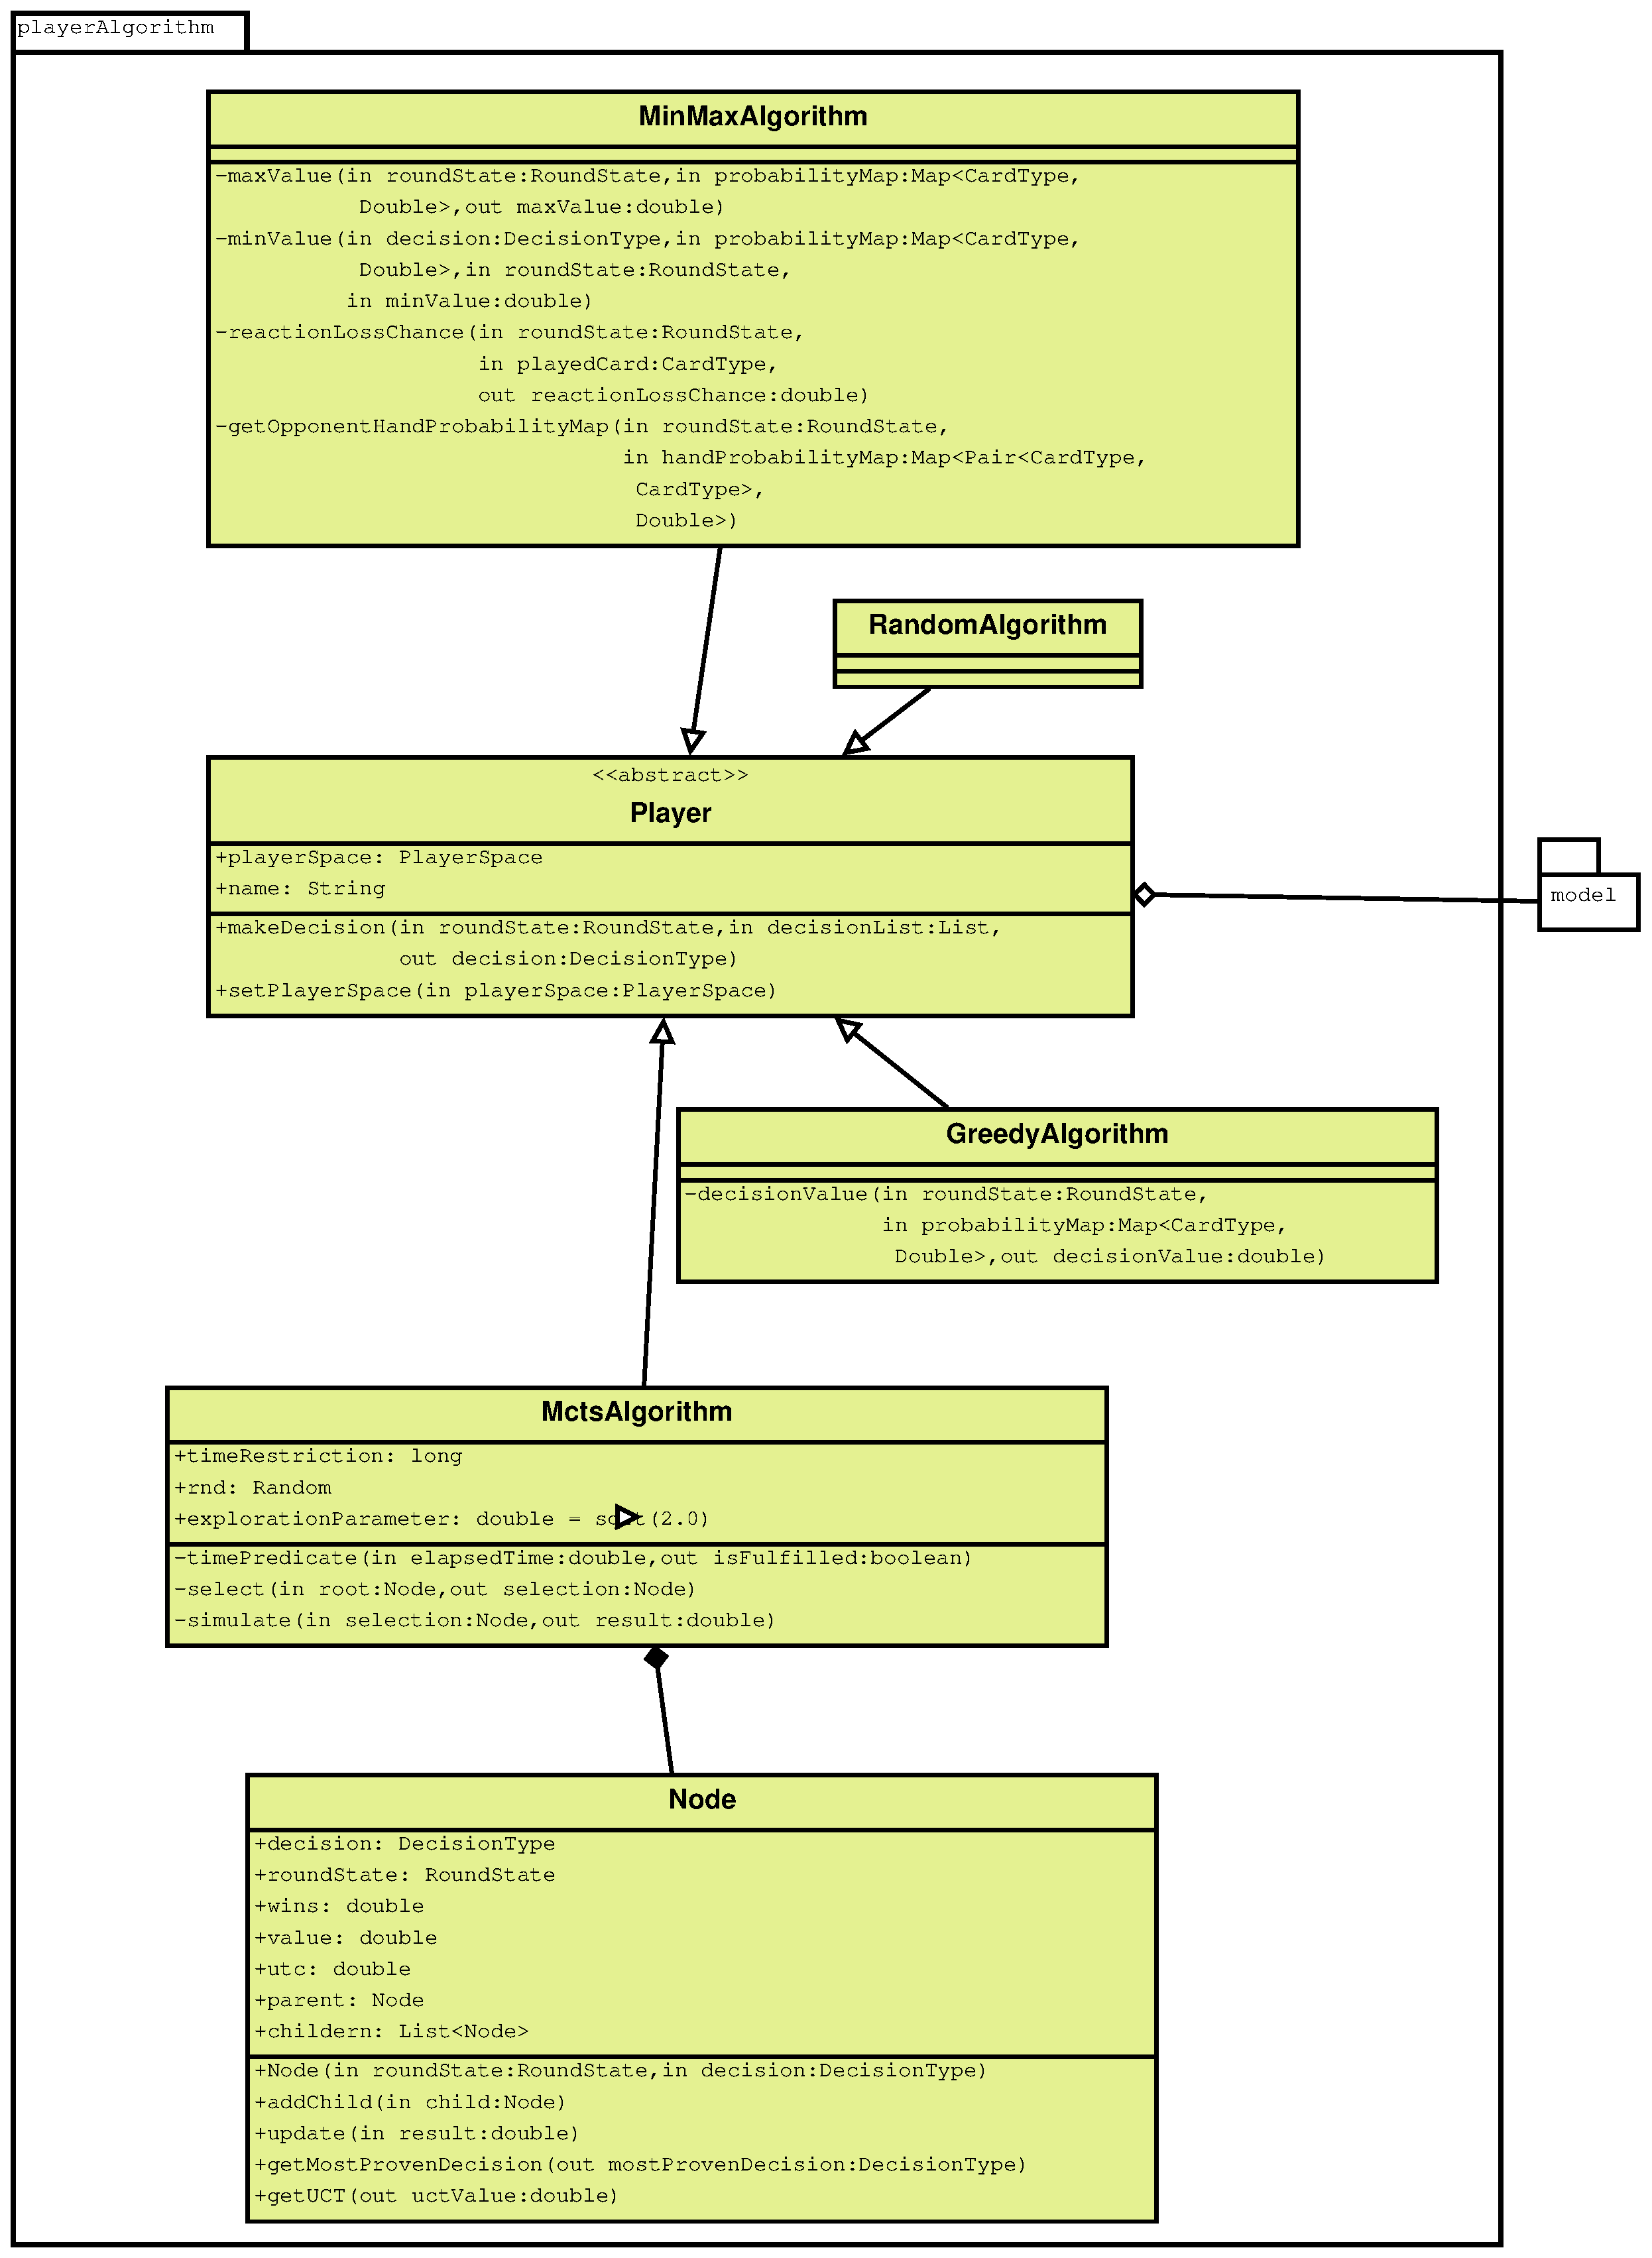
\includegraphics[width=\textwidth]{Resources/diagramKlas_player.eps}
	\caption{Diagram klas pakietu \textit{player}} 
	\label{fig:llMainImage}
\end{figure}

W tym pakiecie głównym elementem jest klasa abstrakcyjna Player, po której dziedziczą implementowane przeze mnie algorytmy. Warto zauważyć, że wykorzystuje również pakiet \textit{model}. Takie polimorficzne rozwiązanie znacznie ułatwia dodawanie kolejnych algorytmów do aplikacji, bez konieczności modyfikowania jej.

\subsection{Diagram klas pakietu engine}

\begin{figure}[H]
	\centering
	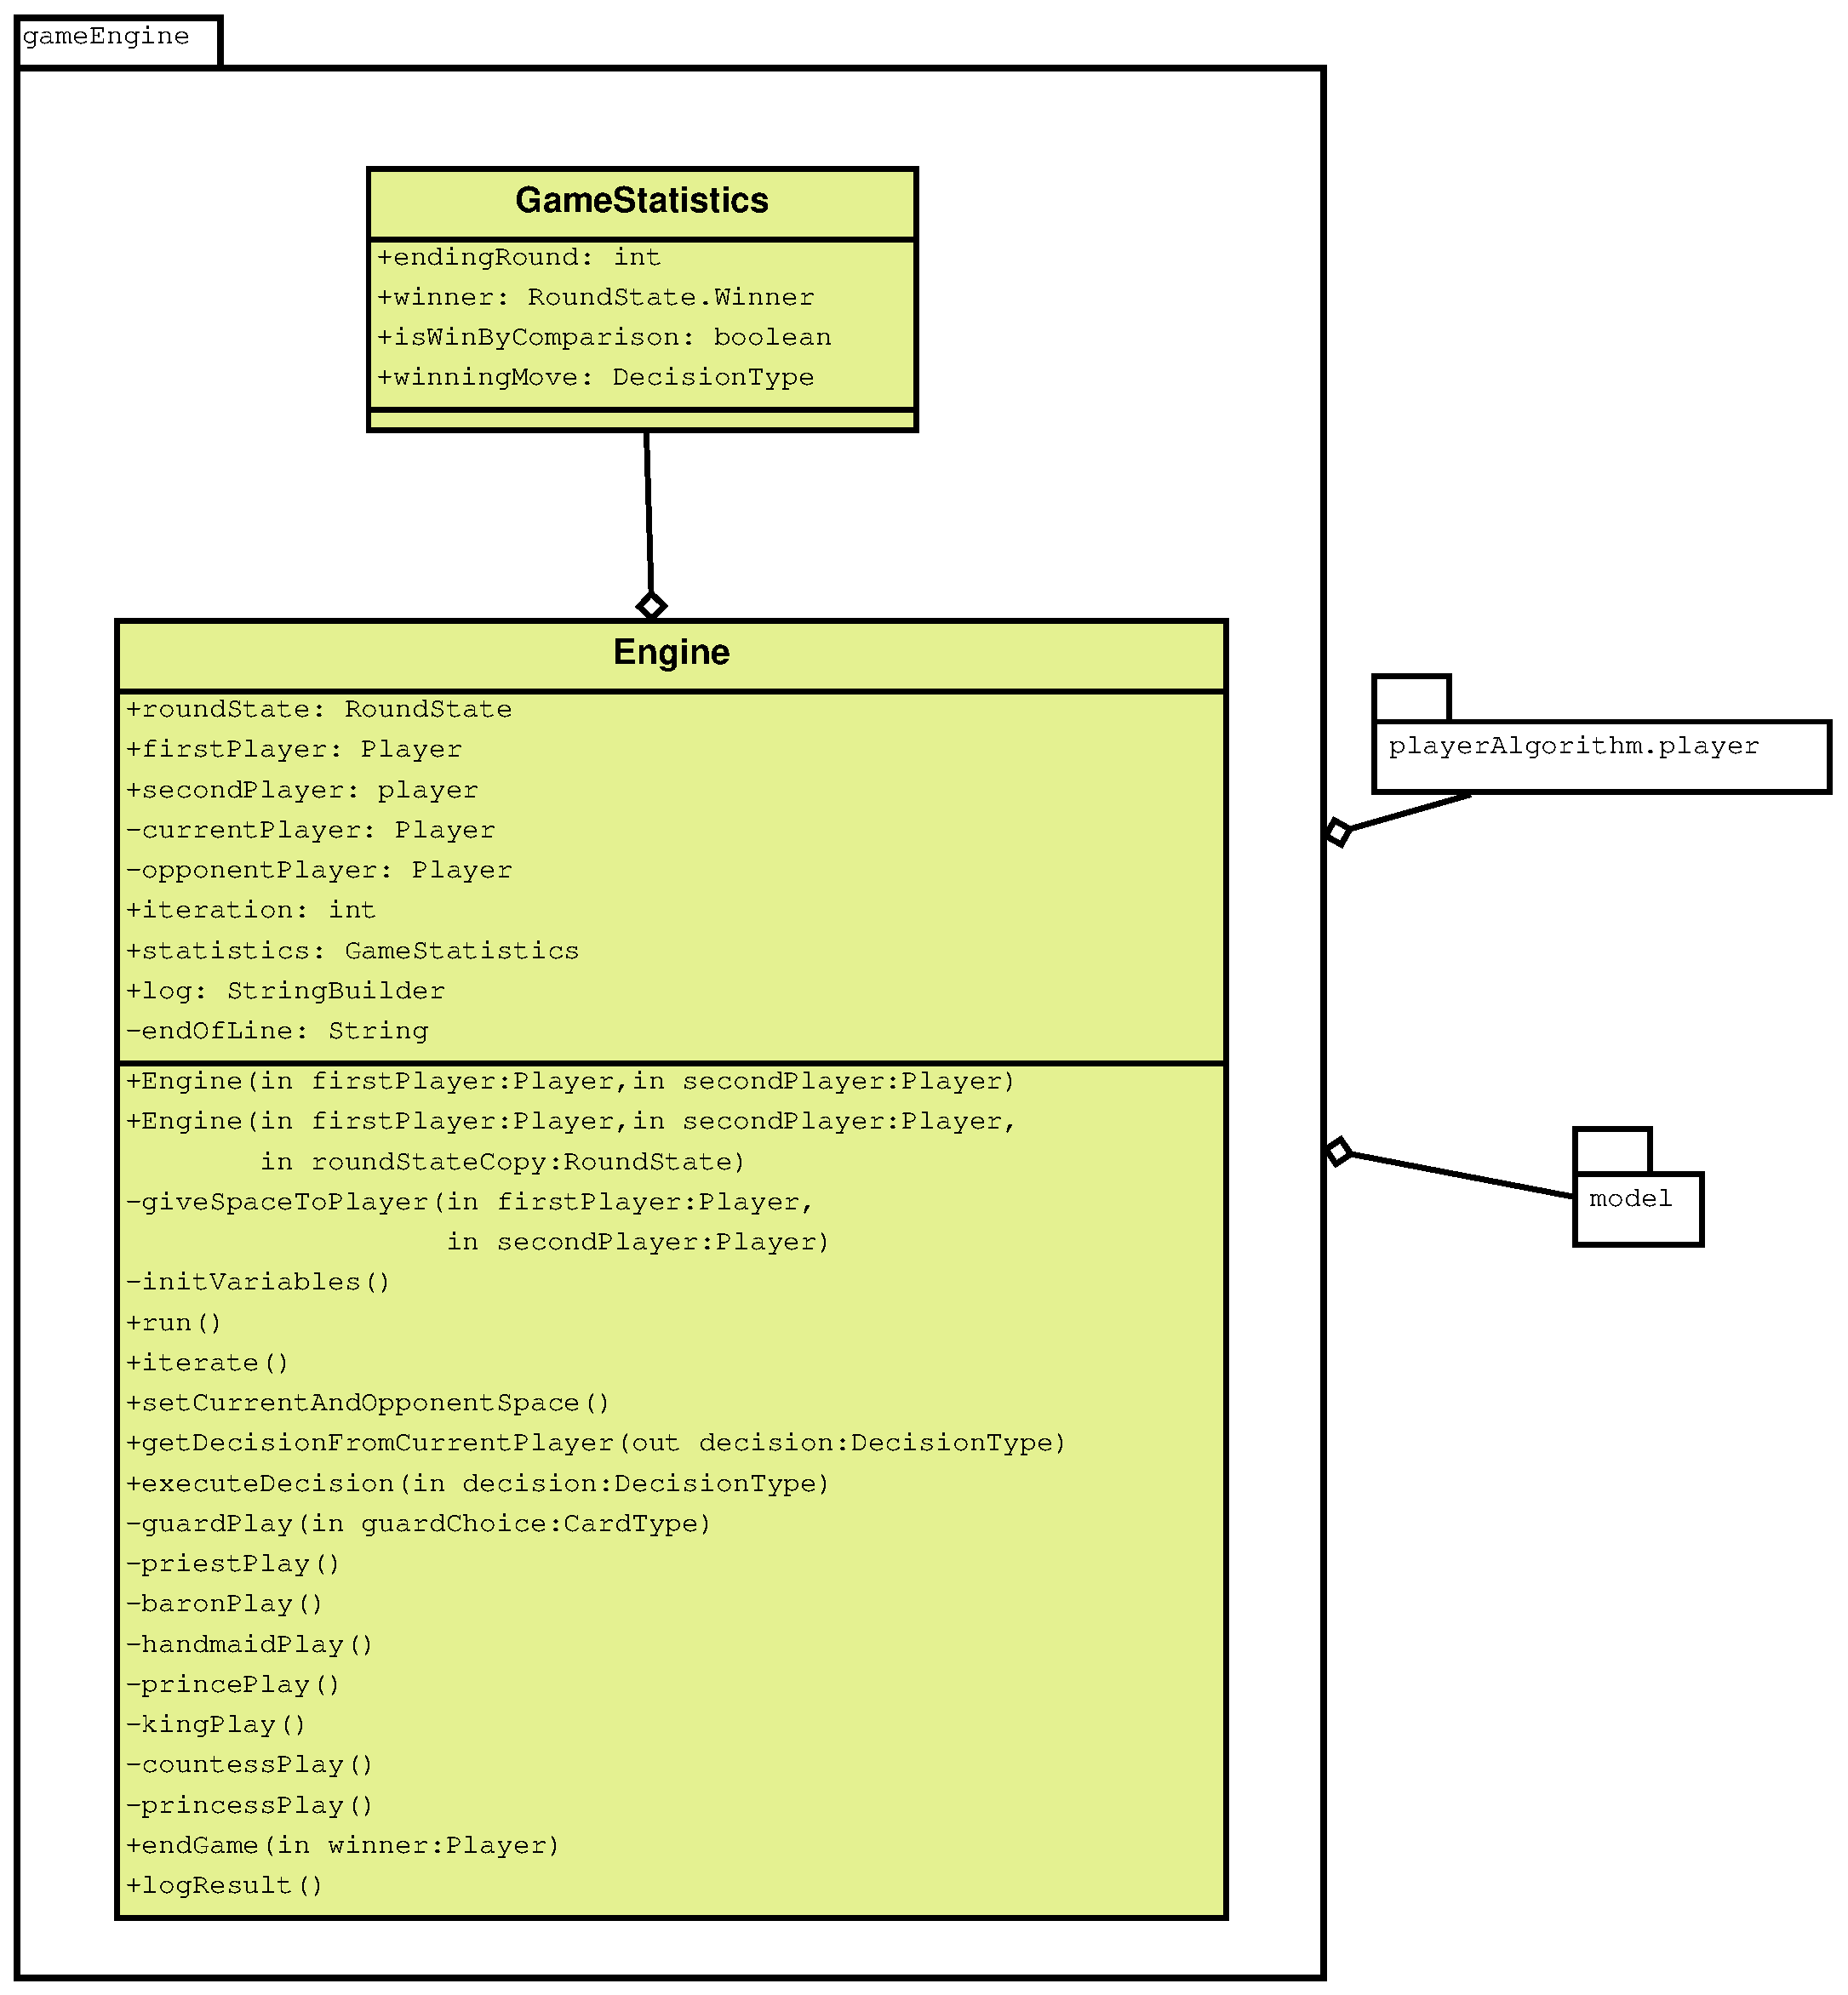
\includegraphics[width=\textwidth]{Resources/diagramKlas_engine.eps}
	\caption{Diagram klas pakietu \textit{gameEngine}} 
	\label{fig:llMainImage}
\end{figure}
Ten pakiet realizuje zasady gry w sensie mechaniki działania kart. Klasa \textit{Engine} jest menadżerem i zarządza stanem gry na podstawie decyzji otrzymanej z klasy \textit{Player}. Metoda \textit{giveSpaceToPlayer} przekazuje obiektom klasy \textit{Player} referencję do \textit{PlayerSpace} i kopię obiektu \textit{RoundState}. 


\section{Listingi}
Pisząc kod aplikacji, oprócz kierowania się paradygmatami programowania obiektowego, bardzo ważne jest również by dbać o czytelność kodu. W \\ TODO przypis do wujka Boba kod powinien być:
\\TODO uzupełnić cytatem z książki
Kolejną metodologią wspomagającą tworzenie czystego kodu, również autorstwa Boba jest SOLID. Jest to mnemonik opisujący pięć podstawowych założeń programownia obiektowego [\\ TODO przypis wiki]. SOLID oznacza:
\begin{itemize}
	\item S (Single responsibility principle) - Klasa powinna posiadać jedną odpowiedzialność
	\item O (Open/closed principle) - Zmiana wymagań wobec aplikacji nie powinna w konsekwencji zmieniać kodu, lecz dodawać nowe funkcjonalności bez usuwania starych.
	\item L (Liskov substitution principle) - W przypadku dziedziczenia, klasy pochodne muszą mieć możliwość realizacji funkcji klasy bazowej.
	\item I (Interface segregation principle) - Klient nie może być uzależniony od nieużywanego przez niego interfejsu.
	\item D (Dependency inversion principle) - Funkcjonalność wysokopoziomowych modułów nie może zależeć od sposobu działania modułów niskopoziomowych.
\end{itemize}

\subsection{}
\begin{lstlisting}[language=java,label=lst:harris_module,caption=Deklaracja modułu detekcji narożników na obrazie metodą Harrisa]
public void run(){
    do{
	    iterate();
    }while(roundState.turnState != RoundState.TurnState.ended);
    logResult();
}
    
public void iterate(){
    setCurrentAndOpponentSpace();
    roundState.drawCardForPlayerSpace(currentPlayer.playerSpace);
    
    DecisionType decision;
    decision = getDecisionFromCurrentPlayer();
    executeDecision(decision);
    
    
    statistics.winningMove = decision;
    if( roundState.deck.size() == 0 && roundState.turnState != RoundState.TurnState.ended){
	    endGame(null);
	    return;
    }
    roundState.switchState();
    iteration++;
}
    
public DecisionType getDecisionFromCurrentPlayer(){
    return currentPlayer.makeDecision(new RoundState(roundState, currentPlayer.playerSpace), DecisionType.getDecisions(currentPlayer.playerSpace.hand));
}
        
\end{lstlisting}



\section{Prezentacja systemu}
listing kodu mcts
listing kodu silnika
screeny cli z ustawionymi parametrami
screeny z wykresow - w ktorej rundzie sie skonczyla, jakie zagranie najczesciej konczy gre, jaki jest procent zwyciestw (3 wykresy)

\section{Problemy napotkane w trakcie realizacji}
unit testy podczas gdy wiele parametrow jest losowanych
interfejs copy javy - kopiowanie wymaga duzo testow
zle zaplanowany model, gdzie decyzje nie maja dodatkowej klasy. doprowadza to do bardzo duzych switchy